% Uncomment for handout
%\def\HANDOUT{}


\ifdefined\HANDOUT
\documentclass[handout]{beamer}
\usepackage{pgfpages}
\pgfpagesuselayout{4 on 1}[letterpaper,landscape,border shrink=5mm]
\else
\documentclass{beamer}
\fi

\mode<presentation>
{
  \usetheme{Warsaw}
  \definecolor{sered}{rgb}{0.78, 0.06, 0.18}
  \definecolor{richblack}{rgb}{0.0, 0.0, 0.0}
  \setbeamercolor{structure}{fg=sered,bg=richblack}
  %\setbeamercovered{transparent}
}


\usepackage[english]{babel}
\usepackage[latin1]{inputenc}
\usepackage{times}
\usepackage[T1]{fontenc}
\usepackage{tikz}
\usepackage{graphicx}
\usepackage[export]{adjustbox}
\usepackage{fancyvrb}
\usepackage{amsmath}
\usepackage{amssymb}
\usepackage{esvect}

\makeatletter
\newcommand{\imagesource}[1]{{\centering\hfill\break\hbox{\scriptsize Image Source:\thinspace{\tiny\itshape #1}}\par}}
\newcommand{\image}[3][\@nil]{%
        \def\tmp{#1}%
        \begin{center}
        \ifx\tmp\@nnil
            \includegraphics[max height = 0.55\textheight, max width = \textwidth]{images/#2}
        \else
            \includegraphics[max height = 0.50\textheight, max width = \textwidth]{images/#2}
            \linebreak
            #1
        \fi
        \linebreak
        {\tiny Image Source:\thinspace{\tiny #3}}
        \end{center}
}

\newenvironment{code}{%
 \VerbatimEnvironment
 \begin{adjustbox}{max width=\textwidth, max height=0.7\textheight}
 \begin{BVerbatim}
  }{
  \end{BVerbatim}
 \end{adjustbox}
}


\newenvironment{scaled}{%
 \begin{adjustbox}{max width=\textwidth, max height=0.7\textheight}
 }{
 \end{adjustbox}
}

\title{Object Oriented Programming with C++}


\author{Robert Lowe}

\institute[Southeast Missouri State University] % (optional, but mostly needed)
{
  Department of Computer Science\\
  Southeast Missouri State University
}

\date[]{}
\subject{}

\pgfdeclareimage[height=1.0cm]{university-logo}{images/semo-logo}
\logo{\pgfuseimage{university-logo}}



\AtBeginSection[]
{
  \begin{frame}<beamer>{Outline}
    \tableofcontents[currentsection]
  \end{frame}
}


\begin{document}

\begin{frame}
  \titlepage
\end{frame}

\begin{frame}{Outline}
  \tableofcontents
\end{frame}


% Structuring a talk is a difficult task and the following structure
% may not be suitable. Here are some rules that apply for this
% solution: 

% - Exactly two or three sections (other than the summary).
% - At *most* three subsections per section.
% - Talk about 30s to 2min per frame. So there should be between about
%   15 and 30 frames, all told.

% - A conference audience is likely to know very little of what you
%   are going to talk about. So *simplify*!
% - In a 20min talk, getting the main ideas across is hard
%   enough. Leave out details, even if it means being less precise than
%   you think necessary.
% - If you omit details that are vital to the proof/implementation,
%   just say so once. Everybody will be happy with that.

\section{Object Oriented Programming}
\begin{frame}{Definitions}
    \begin{description}[<+->]
    \item[Object] An entity which includes state and behavior.
    \item[Class] A group of related objects.
    \item[Object Oriented Programming] A method of modular
        decomposition where a program is decomposed into collections
        of objects which work together to accomplish their task.
    \end{description}
\end{frame}



\begin{frame}{Basic Features of Object Oriented Programming}
    \begin{itemize}[<+->]
        \item {\bf Abstraction} -- Implementation details of each object are hidden.
        \item {\bf Encapsulation} -- Internal state and behavior are packaged into objects.
        \item {\bf Inerhitance} -- Objects can inherit the properties of other objects.
        \item {\bf Polymorphism} -- Code written for more general/abstract objects can operate more concrete classes.
    \end{itemize}
\end{frame}

\begin{frame}{An Example of Inheritance and Polymorphism}
    \begin{itemize}[<+->]
        \item A {\bf squirrel} is a {\bf mammal}.
        \item All {\bf mammals} have fur, give live birth, and feed their young with milk.
        \item Therefore all {\bf squirrel}s have fur, give live birth, and feed their young with milk.
        \item If you build code that knows how to {\bf milk} a {\bf mammal}, it also knows how to {\bf milk} a {\bf squirrel}.
    \end{itemize}
\end{frame}


\begin{frame}{Object Oriented Goals}
    \begin{itemize}[<+->]
        \item {\bf Modular Decomposition} -- Subdivide a program into multiple small segments to manage complexity and provide teamwork.
        \item {\bf Code Reuse} -- Create objects which can be used in other applications.
        \item High Quality OOP Code Exhibits:
            \begin{itemize}
                \item {\bf Loose Coupling} -- Objects depend only on public interfaces.
                \item {\bf High Cohesion} -- Each object has a well-defined purpose.
            \end{itemize}
        \item Poor Quality OOP Code:
            \begin{itemize}
                \item {\bf The ``God Class''} -- A tightly coupled class that controls every aspect of the system.
                \item {\bf The ``Swiss Army Class''} -- A class who's objects can do anything!They print, they store, they act, and more!
            \end{itemize}
    \end{itemize}
\end{frame}


\begin{frame}{How to Write SOLID Code}
    \begin{itemize}[<+->]
        \item {\bf S}ingle Responsibility Principle -- Each class should have just one, well-defined purpose.
        \item {\bf O}pened / Closed Principle -- Classes should be open for extension, but closed for modification.
        \item {\bf L}iskov Subsitution Principle -- Derived classes should be substitutable for their base classes.
        \item {\bf I}nterface Segregation Principle -- Clients should not be forced to depend on interfaces they do not use.
        \item {\bf D}ependency Inversion Principle -- High level modules should not depend on low level modules; both should depend on abstractions.
    \end{itemize}
\end{frame}


\section{An OOP Example}

\begin{frame}{Casino Blackjack}
    \begin{columns}
        \column{0.6\textwidth}
        \begin{itemize}[<+->]
            \item The dealer deals two cards to each player.
            \item The dealer takes one face down card and one face up card.
            \item Number cards (2--10) are worth their face value.
            \item Aces are worth either 1 or 11, whichever is better.
            \item Face cards are (J, Q, K) are worth 10.
            \item Players can take additional cards on their turn.
            \item The object is to get as close to 21 without going over.
        \end{itemize}
        \column{0.4\textwidth}
        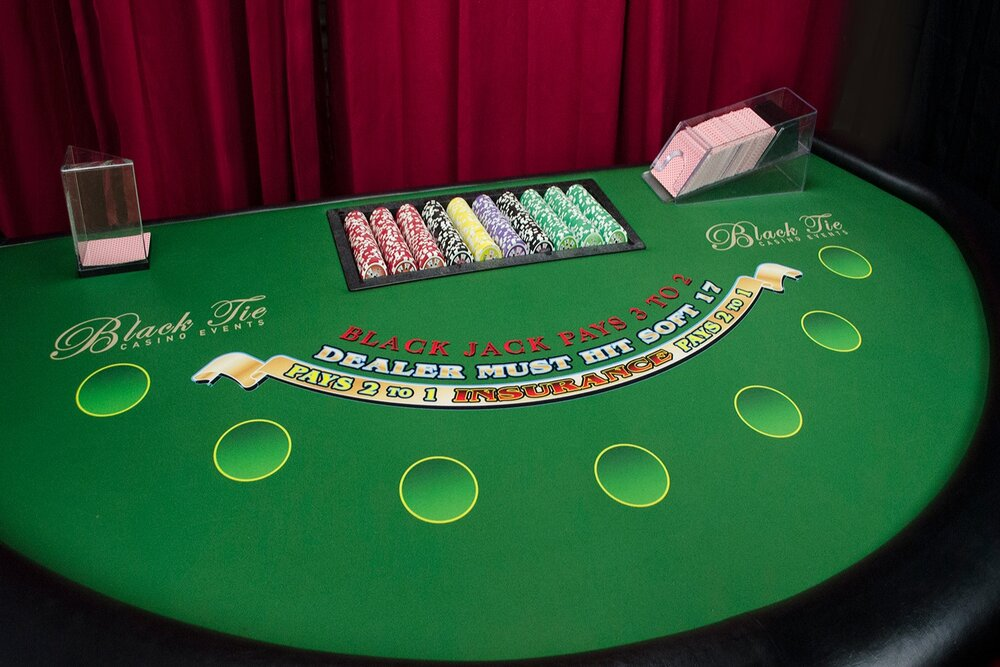
\includegraphics[max width=\textwidth]{images/blackjack}
    \end{columns}
\end{frame}


\begin{frame}[fragile]{The Card Object}
    \begin{code}
class Card 
{
public: 
    Card(const std::string &value, char suit);
    const std::string& value() const;
    char suit() const;

private:
    char _suit;
    std::string _value;
};

std::ostream &operator<<(std::ostream &os, const Card &card);
    \end{code}
\end{frame}

\begin{frame}[fragile]{The Shoe Object}
    \begin{code}
class Shoe
{
public:
    // create a shoe of n decks
    Shoe(int n);

    Card deal();
    
    unsigned int remaining() const;
private:
    std::vector<Card> _contents;       // The contents of the shoe
    std::vector<Card>::iterator _top;  // The top card in the shoe
};
    \end{code}
\end{frame}


\begin{frame}[fragile]{The Hand Object}
    \begin{code}
class Hand 
{
public:
    Hand(const Card &down, const Card &up);

    // get / set revealed status
    bool revealed() const;
    void revealed(bool _revealed);

    // get best point value
    int point() const;

    // get the hard value (with aces 1)
    int hard() const;

    // get soft value (zero if soft busts or no ace)
    int soft() const;

    //receive a hit
    void hit(const Card &card);

    //const iterators for observing hand
    std::vector<Card>::const_iterator begin() const;
    std::vector<Card>::const_iterator end() const;

private:
    std::vector<Card> _cards;
    int _hard;
    int _soft;
    bool _revealed;
};


// Insertion operator to print a hand
std::ostream& operator<<(std::ostream &os, const Hand &hand);
    \end{code}
\end{frame}


\begin{frame}{The Files of the Blackjack Program}
    \begin{itemize}
        \item<2-> {\bf Header Files}
            \begin{itemize}
                \item card.h
                \item hand.h
                \item shoe.h
            \end{itemize}
        \item<3-> {\bf Implementation Files}
            \begin{itemize}
                \item blackjack.cpp
                \item card.cpp 
                \item hand.cpp
                \item shoe.cpp                        
            \end{itemize}
        \item<4-> {\bf Build File}
            \begin{itemize}
                \item Makefile
            \end{itemize}
    \end{itemize}
\end{frame}

\begin{frame}[fragile]{The Makefile}
    \begin{code}
CXXFLAGS=-g --std=c++20

blackjack: blackjack.o card.o shoe.o hand.o
	g++ -o $@ $^ $(CXXFLAGS)

blackjack.o: blackjack.cpp
	g++ -c -o $@ blackjack.cpp $(CXXFLAGS)

card.o: card.cpp card.h
	g++ -c -o $@ card.cpp $(CXXFLAGS)

shoe.o: shoe.cpp shoe.h
	g++ -c -o $@ shoe.cpp $(CXXFLAGS)

hand.o: hand.cpp hand.h
	g++ -c -o $@ hand.cpp $(CXXFLAGS)

clean:
	rm -f *.o blackjack
    \end{code}
\end{frame}

\end{document}
